\pdfoutput=1
\documentclass[a4paper,12pt,titlepage, twoside]{article}
\usepackage[english]{babel}
\usepackage[utf8]{inputenc}
\usepackage{amssymb,amsmath}
\usepackage{algorithm,algpseudocode}
\usepackage[title,titletoc]{appendix}
\usepackage{natbib}
\usepackage{siunitx}
\usepackage{textcomp}
\usepackage[symbol]{footmisc}
\usepackage{booktabs}


\newcommand{\Author}{Zdeněk Rozsypálek}
\newcommand{\Title}{Active 3D mapping using laser range finder with steerable measuring rays}
\newcommand{\Acronym}{Acronym}
\newcommand{\WorkPackage}{WorkPackage}
\newcommand{\DocName}{Thesis}
\newcommand{\Subject}{\WorkPackage - \DocName}
\newcommand{\Keywords}{mobile robotics}
\newcommand{\Date}{1/1/2017}
\newcommand{\DOCVersion}{0.1}
\newcommand{\jed}[1]{\ensuremath{~\mathrm{#1}}} %příkaz pro sazbu fyzikálních jednotek

\def\clinks{false}

\usepackage{latexsym}
\usepackage{a4wide}
\usepackage{color} 
\usepackage{indentfirst}
\usepackage{graphicx}       %%% graphics for dvips
\usepackage{fancyhdr}
\usepackage{longtable}
\usepackage{pifont}
\usepackage{makeidx}
\usepackage{lastpage}
\usepackage{multirow}
\usepackage{dcolumn} 
\usepackage{epstopdf}
\usepackage{url}
\usepackage{listings}
\usepackage{caption}
\usepackage{subcaption}
\usepackage{relsize}
\usepackage{pdfpages}
\usepackage{natbib}
\usepackage{url}

\lstset{breaklines=true,captionpos=b,frame=single,language=sh,float=h}
\lstloadlanguages{sh,c}
\def\lstlistingname{Listing}%{Výpis}
\def\lstlistlistingname{Listings}%{Seznam výpisů}

% European layout (no extra space after `.')
\frenchspacing

% no indent, free space between paragraphs
\setlength{\parindent}{1cm}
\setlength{\parskip}{1ex plus 0.5ex minus 0.2ex}

\usepackage{ifthen} %%% package for conditionals in TeX
\newread\testin
\def\softinput #1 {\let\next=\relax \openin\testin=#1
\ifeof\testin \message{Info: the file #1 does not exist}%
\else \closein\testin \def\next{\input #1 }\fi
\next}

\softinput{makeconfig}

\ifx\clinks\undefined
\def\clinks{true}
\fi

\ifx\pdfoutput\undefined %%% LATEX %%%
\def\nothtml{}  %%% \nothtml is defined if not processed with latex2html
%\usepackage[dvips]{graphicx}       %%% graphics for dvips
\usepackage[                %%% hyper-references for ps2pdf
bookmarks=true,%                   %%% generate bookmarks ...
breaklinks=true,%                  %%% breaks lines, but links are very small
hypertexnames=false,%              %%% needed for correct links to figures
colorlinks=\clinks,%
urlcolor=blue
]{hyperref}           %%% blue instead of cyan URLS
\hypersetup{
pdfcreator  = {LaTeX with hyperref package},
pdfproducer = {dvips + ps2pdf},
}
\else %%% PDFLATEX %%%
\def\nothtml{}  %%% \nothtml is defined if not processed with latex2html
%\usepackage[pdftex]{graphicx}        %%% graphics for pdfLaTeX
\usepackage[              %%% hyper-references for pdflatex
bookmarks=true,%                   %%% generate bookmarks ...
hypertexnames=false,%              %%% needed for correct links to figures
breaklinks=true,%                  %%% break links if exceeding a single line
colorlinks={\clinks},%
urlcolor=blue]{hyperref}           %%% blue instead of cyan URLS
\pdfadjustspacing=1                %%% force LaTeX-like character spacing
\fi

\hypersetup{  
pdfauthor={\Author},
pdftitle={\Title - \Acronym},
pdfsubject={\Subject},
pdfkeywords={\Keywords}
}

\def\BackgroundEPS#1#2#3#4{%
\special{ps: @beginspecial @setspecial initmatrix
0.1 setgray #2 #3 translate #4 dup scale}
\special{ps: plotfile #1}
\special{ps: @endspecial}
}

\pagestyle{fancy}
\setlength{\headheight}{18pt}
\renewcommand{\footrulewidth}{0.4pt}

%\lfoot{ČVUT FEL, Katedra Kybernetiky, Gerstner Laboratory}
\cfoot{}
%\rfoot{\thepage$/$\pageref{LastPage}}

\fancypagestyle{plain}

\fancyhead[R]{}

\newcommand{\DocBegin}{
\ifx\glreport\undefined
\else
\input{../common/glreport}
\fi
}


\renewcommand{\lstlistlistingname}{List of Algorithms}
\renewcommand{\lstlistingname}{Listing}
\definecolor{background_color}{rgb}{1.0, 1.0, 0.85}
\definecolor{comment_color}{rgb}{0.0, 0.5, 0.0}
\definecolor{keyword_color}{rgb}{0.0, 0.0, 1.0}
\definecolor{string_color}{rgb}{0.8, 0.0, 0.0}
\lstset{language=ksh}
\lstset{backgroundcolor=\color{background_color}}
\lstset{frameround=tttt}
\lstset{columns=fullflexible}
\lstset{keywordstyle=\color{keyword_color}\bfseries}
\lstset{commentstyle=\color{comment_color}}
\lstset{stringstyle=\color{string_color}}
\lstset{basicstyle=\ttfamily}
\lstset{showstringspaces=false}
\lstset{frame=single}
\lstset{keepspaces=true}
\lstset{tabsize=4}
\lstset{breaklines=true}
\lstset{captionpos=b}

\begin{document}
\DocBegin
%% Asymetric margins
%% LEAVE ONLY IN THE PRINTED VERSION !!!!!!!!!!!!!!!!!!!!!!!!!!!!!!!!!!!!!!!!!!!!!!!!!!!!!!!!!!!!!
%% the electronic version should have symetric margins
%\setlength{\oddsidemargin}{+0.5cm} 
%\setlength{\evensidemargin}{-0.5cm}
%%

% Titulní stránka
\begin{titlepage}
\begin{center}

{\Large CZECH TECHNICAL UNIVERSITY IN PRAGUE}
\vskip 10pt

\vskip 8pt
{\Large Faculty of Electrical Engineering}
 
%\vskip 0pt plus 2fill
\vspace{50pt}
{\Huge\bf BACHELOR'S THESIS}\\
\vspace{40pt}
\includegraphics[width=10cm]{fig/lev.pdf}

\vspace{40pt}
{\Large\rm \Author } \\
\vspace{20pt}
{\Large\bf \Title}

\vspace{60pt}
{\bf Department of Cybernetics}\\
\vspace{5pt}   
{Thesis supervisor: {\bf Ing. Tomáš Petříček}}

\vspace{30pt}
%{\sc Prague 2013}
\end{center}
\end{titlepage}

\pagestyle{empty}
\cleardoublepage

\includepdf[pages={1}]{acknowledgement.pdf}
\cleardoublepage

\includepdf[pages={1}]{zav_prace.pdf}
\cleardoublepage

~\vfill{}

\section*{Acknowledgements}

I would like to thank my adviser for his advice.

\vspace{2.5cm}

\newpage{}

\cleardoublepage % it is prefered for the 1. level sections to start on the 

\vfill
\begin{center}
{\it \large Abstract}
\vspace{0.2cm}

\begin{minipage}{0.8\textwidth}{
Bakalářská práce se zaměřuje na ovládání \textit{solid-state} lidarů s omezeným počtem natáčecích paprsků. Kromě plánování směrů paprsků se práce věnuje i rekonstruování 3D mapy z řídkých měření těchto lidarů. V práci se pro rekonstruování a plánování používají hluboké neuronové sítě. Plánovací část využívá \textit{reinforcement learning} metody pro trénink neuronových sítí. Bylo vytvořeno trénovací prostředí implementující framework pro trénování \textit{reinforcement learning} agentů. Za pomocí stochastických metod se podařilo navrhnout agenta, který nabízí dostatečnou škálovatelnost a překonává náhodný plánovač.
}
\end{minipage}
\end{center}
\vfill
\vspace{1cm}

\vfill
\begin{center}
{\it \large Abstrakt}
\vspace{0.2cm}

\begin{minipage}{0.8\textwidth}{
Bachelor thesis aims at control of the solid-state lidar sensor with a limited number of steerable rays. Besides planning the directions of the rays, thesis is also devoted to creating a dense 3D maps from a sparse measurements. The theses use a deep neural networks for planning the rays and reconstructing the dense maps. Planning part exploits the reinforcement learning concept for training of the neural network. An environment implementing the framework for training of the reinforcement learning agents was created. The agent, proposed in this thesis, is using stochastic methods to achieve sufficient scalability in the challenging environment.
}
\end{minipage}
\end{center}
\vfill
\vspace{1cm}
\newpage{}

\cleardoublepage

\pagenumbering{roman}
\cfoot{\thepage}

\tableofcontents
\cleardoublepage

\listoffigures
\cleardoublepage


\pagestyle{fancy}
\fancyhf{}
\pagenumbering{arabic}
\cfoot{}
\fancyfoot[RO,RE]{\thepage$/$\pageref{LastPage}}
\setlength{\parskip}{0.35cm}

\fancyhead[LO,LE]{INTRODUCTION}
\section{Introduction}

Lidar sensors offer an accurate volumetric mapping of surrounding space. There is much utilization of volumetric space reconstructions in different fields. For example, lidar sensors are nowadays essential equipment for a large variety of autonomous vehicles. The sensor can help autonomous vehicles to orientate in an environment. One of the most significant issues which prevent broader implementation of these sensors is a relatively high price. Breakthrough in this field is solid-state lidars. These lidars do not have moving parts, and their price should be circa hundreds of dollars \cite{quanergy2016}. The major drawback of this sensor is a limited number of rays which can be sent over the certain time frame and only in chosen directions. Zimmermann et al. \cite{zimmermann2017} proposed mapping agent which creates dense reconstructions from sparse measurements. They also proposed prioritized greedy planning for choosing directions of these rays. The objective of this thesis is to apply reinforcement learning (RL) methods to learn planning of the rays and contribute to methods of controlling these sensors. RL is a field of study based on concepts of behavioral psychology, especially the trial and error method, and has in recent years experienced a rapid development due to the growth of computational power and neural networks improvement. Richard Sutton has made a helpful summary of RL concepts in his book \cite{sutton2012}. One of the biggest achievements was playing Atari games by a RL agent without any prior knowledge of the environment \cite{mnih2015}. Soon after the RL agent, able to solve simple continuous problems such as balancing inverse pendulum on a cart, was introduced. Today state-of-the-art methods can solve complex environments with infinite action spaces. Although these methods reach great successes, they still suffer from lack of sample efficiency - they need for training many episodes before environment can be solved. This inefficiency makes creating agent controlling lidar very challenging, since training large neural networks is very time-consuming. The agent is divided into two parts - mapping and planning. The mapping part should create a best possible reconstruction from sparse measurements, while the planning part is focused on picking rays that will maximize reconstruction accuracy. Agents are trained using a publicly available dataset which contains drives of a car equipped with Velodyne lidar \cite{geiger2013}. Theoretical background of RL is discussed in first part of this thesis. In the second part are methods from first part used to solve the Lidar-gym environment \cite{rozsypalek2018}.
  
\clearpage

\fancyhead[LO,LE]{THEORETICAL BACKGROUND}
\section{RL basics}
Firstly, environment where an agent is able operate must be defined. Environment can be described as Markov decision process, where $S_t \in \mathcal{S}$ is a state from a set of possible states $\mathcal{S}$ in which environment is located in time $t$. Agent can observe the state of the environment and take action accordingly. Action is a transition between states. Every action $A_t \in \mathcal{A}$ moves the environment from $S_t$ to $S_{t+1}$. The environment evaluates every action and returns appropriate reward $R_t$. In RL set $\mathcal{A}$ is often called action space and set $\mathcal{S}$ observation space. The main goal of the agent is to maximise a expected reward.

\begin{figure}[!h]
\centering
\includegraphics[scale=0.3]{fig/RL-concept.png}
\caption{RL concept}
\end{figure}

Major issue is that maximising immediate reward is often not an effective approach to maximising the overall reward. This greedy policy can take the agent into very disadvantageous state. Thus, the agent must take into account future states and rewards. In the past agents used to contain big tables which stored information about the quality of every action in every state. This is possible in environments with small action and observation spaces but is very memory consuming for larger environments and even impossible for continuous action or observation space. Therefore, modern methods use neural networks as function estimators.

\subsection{Temporal difference learning}
Temporal difference (TD) learning combines the ideas of Monte Carlo methods and dynamic programming. It is able to learn directly from experience obtained by interactions with an environment without any prior knowledge of said environment. TD learning is done by following an assignment in each timestamp [Sutton]
\begin{equation}
V(S_t) \gets V(S_t) + \alpha [R_{t} + \gamma V(S_{t+1}) - V(S_t)]
\end{equation}
where $V$ is so called state value, which shows how good is being in a particular state with the current policy. $\alpha \in \mathbb{R}^+$ is step size and $\gamma \in (0, 1)$ is discount factor.

\subsection{Q-learning}
Q-learning is type of TD learning developed by Watkins [1989]. The state value $V$ from previous subsection is replaced by $Q$ value, which refers to quality of action in a particular state instead of quality of the state itself. When we rewrite TD learning (1) to Q-learning we get:
\begin{equation}
Q(S_t, A_t) \gets Q(S_t, A_t) + \alpha [R_{t} + \gamma \underset{A_{t+1}}{max} Q(S_{t+1}, A_{t+1}) - Q(S_t, A_t)].
\end{equation}
Our policy here is to take action with maximal $Q$ value. That is called greedy policy. Obvious drawback of greedy policy is that it does not allow to explore the whole environment properly because an action with the highest $Q$ value is always chosen. A solution to this problem is sometimes take random action to explore the environment. This policy is often referred to as $\epsilon$-greedy policy.

\begin{algorithm}
\caption{$\epsilon$-greedy policy}\label{euclid}
\begin{algorithmic}[1]
\Procedure{ChooseAction}{}
\State $\epsilon \gets \epsilon \cdot \epsilon_d$
\If {$\epsilon >$ random $\in (0,1)$}
\State action $\gets$ random $\in \mathcal{A}$
\Else 
\State action $\gets$ $\underset{A_t}{max} Q(S_t, A_t)$
\EndIf
\State \Return action
\EndProcedure
\end{algorithmic}
\end{algorithm}

It is common to set $\epsilon = 1$ at the beginning of the training and decay rate $\epsilon_d$ close to one. This policy assumes that it is needed to explore an environment first and then exploit agents experience.

\clearpage
\section{Deep neural networks in RL}
As was stated in previous chapter, tabular methods are very inefficient in large environments. In these instances deep neural networks which can replace tables come into effect. Deep Q networks (DQN) proposed by Google’s Deepmind [2015] outperformed all previous RL algorithms in playing Atari games. With neural networks, also grew the popularity of policy gradient methods [Sutton], where neural network outputs a specific action instead of Q values. Note that the most of these methods are general and not necessarily tied to neural networks.

\subsection{Deep Q network}
Neural network takes current state as input and outputs Q value for each possible action. Network is trained using gradients of Q value in current state with respect to trainable weights $\theta$ of our neural network.
\begin{align}
\delta_t &= R_{t} + \gamma \underset{A_{t+1}}{max}Q^\theta(S_{t+1}, A_{t+1}) - Q^\theta(S_t, A_t)\\
\theta_{t+1} &= \theta_t + \alpha \delta_t \nabla_\theta Q^\theta (S_t, A_t).
\end{align}
We are updating gradients in proportion to TD $\delta_t$. Unfortunately, this simple DQN agent suffers from a lack of sample efficiency and does not converge well. There are many techniques which can help DQNs to achieve satisfying results.

\subsection{Target network}
Target network is a technique proposed by Mnih[Citace] to improve convergence of DQN learning. It uses two neural nets instead of one. The first is trained online network on a batch of data and the second target network is used for predictions during training. After the completion of training on a batch of data, the target network is updated
\begin{equation}
\theta^- = \tau \theta + (1-\tau)\theta^-
\end{equation}
where $\theta^-$ is set of trainable weights of the target network, $\theta$ indicates online network weights and $\tau << 1$ is constant.
TD $\delta$ is now calculated using target network:
\begin{equation}
\delta_t = R_{t} + \gamma \underset{A_{t+1}}{max}Q^{\theta^-}(S_{t+1}, A_{t+1}) - Q^\theta(S_t, A_t). 
\end{equation}
Target network stabilises training since predicting network does not change after each training step.

\subsection{Prioritized experience replay}
Experience replay is biologically inspired mechanism introduced by [Schaul-citace] which stores all experiences (specifically: $S_t$, $A_t$, $R_{t}$, $S_{t+1}$) into a buffer and assigns priority to every experience. Main idea is that experiences with high TD should have higher priority. Thus is necessary to calculate priority $p$ from TD error:
\begin{equation}
p = (|\delta_t | + \beta)^\alpha
\end{equation}
where $\alpha$ indicates how much we prefer experiences with higher priority and $\beta << 1$ is a constant which helps to avoid priorities very close to zero. Considering a greedy selection would abandon experiences with low priority, a better approach is to choose experience $i \in \mathcal{I}$ with probability:
\begin{equation}
P(i) = \frac{p_i}{\sum_{j \in \mathcal{I}} p_j}
\end{equation}
where $\mathcal{I}$ is set of all experiences in the buffer. It is possible now to sample a batch of experiences for training using this probability. It removes correlation in the observation sequence and improves sample efficiency of DQN. It is feasible to store all experiences in a buffer sorted by priority but a more efficient implementation is a sum tree.

\subsection{Double Q-learning}
Classic Q-learning algorithm tends to overestimate actions under certain conditions. Hasselt et al [citace] propose idea of Double Q-learning which decompose the max operation into action selection and action evaluation. Target value is then computed by following equation.
\begin{equation}
Y = R_{t} + \gamma Q(S_{t+1}, argmax_{A_{t+1}}Q(S_{t+1}, A_{t+1};\theta);\theta^-).
\end{equation}
Double DQN outperforms DQN in terms of value accuracy and in terms of policy quality.

\clearpage
\section{Policy gradient}
By this section the goal of neural network was predicting values on the basis of which we determined the policy. In policy gradient method neural network approximates the policy itself. 
\begin{equation}
\theta_{t+1} = \theta_t + \alpha \widehat{\nabla J(\theta_t)}
\end{equation}
where $J$ is performance measure with respect to our neural network parameters and $\widehat{\nabla J(\theta_t)}$ is stochastic estimate which approximates gradient of performance measure. In other words, this method is basically doing stochastic gradient ascent of $J$ with respect to $\theta$ [Sutton]. Policy gradient methods are outperforming DQNs especially in continuous action spaces, because their output is directly continuous action instead of Q-value for every possible action.

\subsection{Actor-Critic}
Thanks to predicting action directly, we gain possibility to predict in continuous action space, but we lost the Q-value which assessed the advantage of action in certain state. That it why the Actor-Critic framework was created. It uses two separate neural networks - Actor which predicts action and Critic which asses action advantage and usually predicts the Q-value of action.
\begin{figure}[!h]
\centering
\includegraphics[scale=0.55]{fig/actor-critic.png}
\caption{Actor-Critic framework}
\end{figure}
\clearpage

\subsection{Deterministic policy gradients}
Deep deterministic policy gradient (DDPG) is one of methods exploiting the Actor-Critic framework. Before DDPG was common practice to use stochastic actor, which predicts parameters of distribution (usually normal distribution). Action of stochastic actor is then a random sample from predicted distribution. Whereas deterministic actor uses distribution sampling only for exploration of action space. We denote $\theta$ and $\omega$ for trainable weights of actor and critic, respectively. Critic update is very similar to DQN:
\begin{align}
\delta_t &= r_t + \gamma Q^\omega(S_{t+1}, \mu ^\theta (S_{t+1})) - Q^\omega(S_t, A_t)\\
\omega_{t+1} &= \omega_t + \alpha \delta_t \nabla_\omega Q^\omega(S_t, A_t).
\end{align}
Note that instead of $A_{t+1}$ is now used function $\mu^\theta(S)$, which is an action estimate by actor neural network. Actor update rule is not so straightforward. 
\begin{equation}
\theta_{t+1} = \theta_t + \alpha\nabla_\theta \mu_{t+1}^\theta(S_t)\nabla_a Q^\omega (S_t, A_t)|_{a = \mu^\theta(S_t)}.
\end{equation}
This equation uses chain rule for derivatives to obtain gradient of Q-values with respect to trainable weights $\theta$. To be explicit:
\begin{equation}
\frac{\partial Q^\omega(S_t, A_t)}{\partial \theta} = \frac{\partial Q^\omega(S_t, A_t)}{\partial A_t} \frac{\partial A_t}{\partial \theta}.
\end{equation}
DDPG significantly outperforms its stochastic counterparts, especially in big continuous action spaces[Silver 2014].

\subsection{Wolpetinger policy}
Actor-Critic methods and DDPG works well in continuous action spaces, but there is a lot of problems with large discrete action spaces, such as recommender systems or lidar planning. Wolpetinger policy is approach how to utilize DDPG in discrete action space [Dulac 2016]. Actor doesn't predict action directly, but it predicts so called proto-action $\tilde{A_t}$.
\begin{equation}
\tilde{A_t} = \mu^\theta(S_t).
\end{equation}
Proto action mostly isn't valid action $\tilde{A_t} \notin \mathcal{A}$. Thus it is necessary to find valid action corresponding to proto action. This is done by computing euclidean distance to every possible action.
\begin{equation}
\mathcal{A}_{knn} = \underset{a \in \mathcal{A}}{argmin}^N | a - \tilde{A_t} |_2 .
\end{equation}
Usually policy choose $N$ closest action to the proto action. $\mathcal{A}_{knn}$ is the set of closest action to proto action. Whole set is then assessed by critic and action with highest Q-value is finally picked.
\begin{equation}
A_t = \underset{a \in \mathcal{A}_{knn}}{argmax} Q^\omega(S_t, a)
\end{equation}
\begin{figure}[!h]
\centering
\includegraphics[scale=0.4]{fig/wolpetinger-policy.png}
\caption{Wolpetinger policy}
\end{figure}
\clearpage

\fancyhead[LO,LE]{EXPERIMENT}
\section{Experiment}
The experiment aims at using reinforcement learning algorithms for controling solid-state lidar with limited number of steerable rays. For purposes of the experiment it was neccessary to implement environment, where an agent can learn and be evaluated \cite{rozsypalek2018}. The lidar-gym environment is written in Python 3 based on OpenAI gym interface \cite{openai2016}. It uses point clouds from the KITTI dataset drives\cite{geiger2013}. One episode of learning in the environment corresponds to one drive in the KITTI dataset. Large point clouds from drives are processed into 3D voxel maps by C++ package \cite{petricek2017}, which also provides ray tracing engine for the environment. Every voxel map is a 3D array containing real numbers which correspond to the occupancy confidence $c$ of each voxel.
\begin{align}
\begin{split}
c &> 0 \quad \text{occupied voxel} \\
c &= 0 \quad \text{unknown occupancy} \\
c &< 0 \quad \text{empty voxel.}
\end{split}
\end{align}

\subsection{Environments}
Lidar-gym implements several environments (visualized in Figure \ref{fig:visualization}), which follow the same template with different sizes of voxel maps and action spaces. Observation space is a local cutout of voxel map, which provides occupancies from sensor's sparse measurements. The sensor is located in the quarter of x-axis and half of y-axis and z-axis of a local cutout. Action space is divided into two parts. First part is dense voxel map reconstructed from observations (sparse measurements). The second part of action space are directions of measuring rays. Each ray has own azimuth and elevation. Environment expects directions in the format of a 2D array of booleans, where true means fired ray. Reward function of the environment is negative logistic loss $-L$ \eqref{eq:loglos}. Parameters of environments are described in Table \ref{tab:envs}.

\begin{table}[H]
\centering
\begin{tabular}{|c||c|c|c|} 
\hline
Name of environment     & Large                        & Small                        & Toy                       \\ \hline
Voxel map size [voxels] & 320 $\times$ 320 $\times$ 32 & 160 $\times$ 160 $\times$ 16 & 80 $\times$ 80 $\times$ 8 \\ \hline
Lidar FOV [\textdegree]           & 120 $\times$ 90              & 120 $\times$ 90              & 120 $\times$ 90           \\ \hline
Densitiy of rays        & 160 $\times$ 120             & 120 $\times$ 90              & 40 $\times$ 30            \\ \hline
Lidar range [m]         & 42                           & 42                           & 42                        \\ \hline
Number of rays          & 200                          & 50                           & 15                        \\ \hline
Voxel size [m] & 0.2 & 0.4 & 0.8 \\ \hline
Episode training time [min]\footnotemark{} & 120 & 15 & 1.5 \\ \hline
\end{tabular}
\caption{Description of environments}
\label{tab:envs}
\end{table}

\clearpage

The environments also offers visualization of actions using Mayavi \cite{mayavi2011} and ASCII art. Agents use neural networks as function estimators, which are implemented in Tensorflow \cite{tensorflow2015} and Keras \cite{keras2015}.

\begin{figure}[h!]
\centering
\includegraphics[width=0.8\linewidth]{fig/gt.png}

\vspace{1mm}

\includegraphics[width=0.8\linewidth]{fig/sparse.png}

\vspace{1mm}

\includegraphics[width=0.8\linewidth]{fig/reconstructed.png}

\caption[Environment visualization]{Visualization of the large environment: The first figure is the ground truth map, second is the voxel map of sparse measurements and third figure shows the dense reconstruction. The dense reconstruction in third figure and the rays fired in second picture are made by an agent using the random planner. Some known structures as cars and trees can be seen in the reconstructed map.}
\label{fig:visualization}
\end{figure}
\renewcommand{\thefootnote}{\fnsymbol{footnote}}
\footnotetext[1]{Using GPU Nvidia 1080Ti.}

\clearpage
Due to the high time complexity, all experiments were conducted in toy environment. The RL agents need significantly more training steps than supervised agents. Unlike the RL agents, for supervised agent is known desired output, thus it can be learned by a gradient descent on the loss function between made and desired output. There are RL agents trained for over million timestamps in OpenAI baselines \cite{openai2017}. One drive in the KITTI dataset has on average 200 epochs. All agents were trained and evaluated on different drives from the city category of the dataset.

\subsection{Mapping agent}
The mapping agent is based on work of Zimmermann et al. \cite{zimmermann2017}. It uses a convolutional neural network (CNN) for reconstructing dense map from sparse measurements. 3D convolutional layers are used to learn the features and max-pooling layers to avoid overfitting. Whole CNN architecture is described in Figure \ref{fig:supervised}.
\vspace{3mm}
\begin{figure}[!h]
\centering
\includegraphics[scale=0.6]{fig/supervised.pdf}
\caption[Mapping network architecture]{Input of the supervised mapping agent is voxel map containing sparse measurements. Output is dense reconstruction of the input.}
\label{fig:supervised}
\end{figure}

Gradient descent is made by Adam optimizer \cite{adam2014}. Optimizer uses logistic loss $L$ between ground truth map $Y$ and predicted dense map $\hat{Y}$.
\begin{equation} \label{eq:loglos}
L(Y, \hat{Y}) = \sum\limits_i w_i \log(1 + \exp(-Y_i \hat{Y_i}))
\end{equation}
where $w$ are weights which balance importance of occupied and unoccupied voxels.
\pagebreak
Unfortunately, a naive implementation of this loss function is computationally inconvenient and often cause numerical issues as overflow. To stabilize training, following modified loss was used \cite{matconvnet2015}
\begin{align} 
\begin{split}
a_i &= -Y_i \hat{Y_i} \\
b_i &= \max(0, a_i) \\
L &= \sum\limits_i w_i (b_i + \log(\exp(-b_i) + \exp(a_i-b_i))).
\end{split}
\end{align}
At first, supervised mapping agent with random ray planning is trained. Reconstructions of the supervised agent are then used for training RL planning agents and after that is mapping agent retrained with RL agent picking the rays.
\subsection{Discrete planning agent}
Since the action of the environment $A_t$ for a direction of the rays is 2D binary array, first try is to use a discrete agent. DQN is the most used option for discrete action space, but in this use case, it requires some tweaks. Note that number of possible actions is extremely large. Even in toy environment it is $40\times30 \choose 15$ $\approx 10^{34}$ of actions. Thus it is necessary to emphasize action space exploration. Further arises the problem with the $\epsilon$-greedy policy, because we are unable to process all possible actions and pick one with the biggest Q-value. We consider only one ray as action to resolve this issure. For $K$ rays is TD from \eqref{eq:qlearn} now computed as:
\begin{align} \label{eq:dql}
\begin{split}
q(S_t, A_t) &= \max\limits_{A_t}^K Q^\theta(S_t, A_t)\\
\delta_t &= R_t + \gamma \overline{q}(S_{t+1}, A_{t+1}) - \overline{q}(S_t, A_t)
\end{split}
\end{align}
where $\overline{q}$ is average $Q$ value over $K$ actions with maximum $Q$ values. DQN agent implements all features as Prioritized experience replay, target network, and double Q learning which are described in the theoretical part of this thesis. Exploration is ensured by action space noise. Neural network architecture is described in Figure \ref{fig:dqn}. The agent uses values of parameters shown in Table \ref{tab:params}. The weights are updated via stochastic optimizer Adam with learning rate $\lambda$.

\clearpage
\begin{figure}[!h]
\centering
\includegraphics[scale=0.6]{fig/dql.pdf}
\caption{DQN architecture.}
\label{fig:dqn}
\end{figure}

\clearpage
\subsection{Continuous planning agent}
The discrete action output was substituted by continuous action, which is then mapped into a 2D binary array. This will allow the agent to avoid extremely large discrete action space. Thank to this substitution it is possible to exploit actor-critic framework. The output the of actor is now $2$ by $K$ array where the first row is the elevation and second is the azimuth of each ray. The last layer of the actor-network is tanh function, so its output is an element of $[-1, 1]$. As training method is used DDPG. The neural network architecture is described in the Figure \ref{fig:ddpg}.

\begin{figure}[!h]
\centering
\includegraphics[scale=0.55]{fig/ddpg.pdf}
\caption[DDPG architecture]{Architecture of the actor is on the left side and critic is on the right side. In the middle can be seen shared inputs and outputs.}
\label{fig:ddpg}
\end{figure}

\pagebreak
To explore action space in our experiments correctly, it is necessary to apply Ornstein-Uhlenbeck random process. When only Gaussian noise is added, actions tend to converge into the corners very fast as in Figure \ref{fig:expdiff}. For actor's and critic's neural network is used Adam optimizer with learning rates $\lambda_{a}$, $\lambda_{c}$. The target networks are used to stabilize learning of actor and critic. The continuous agent also uses prioritized experience replay.

\begin{figure}[H]
\begin{subfigure}[h]{0.5\linewidth}
\includegraphics[width=\linewidth]{fig/wrong_action.eps}
\end{subfigure}
\hfill
\begin{subfigure}[h]{0.5\linewidth}
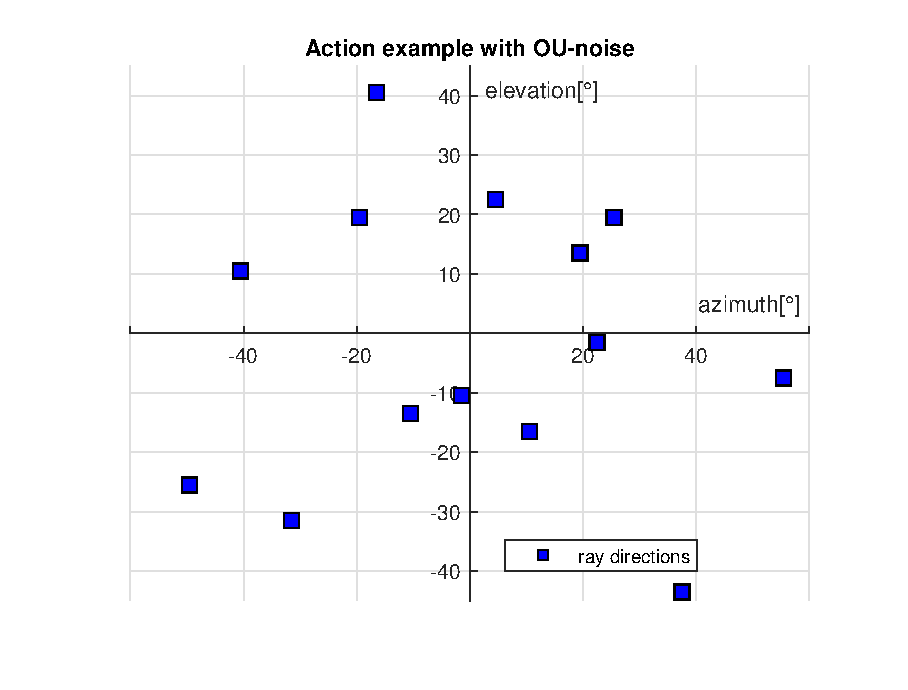
\includegraphics[width=\linewidth]{fig/right_action.eps}
\end{subfigure}
\captionsetup{width=1\textwidth}
\caption[Difference between exploration methods]{Difference between actions made by agents with different exploration methods. Left figure is an example of action made by an agent with Gaussian noise used for exploration. The action in the right figure is taken by agent trained using Ornstein-Uhlenbeck noise.}
\label{fig:expdiff}
\end{figure}

\subsection{Stochastic planning agent}
There is an obvious issue with the deterministic actor. For efficient exploring of ground truth map, it is required to hit as many unique voxels as possible. Thus making several similar actions in a row is not a good strategy. Unfortunately, except first few epochs of every drive, there is not a big difference between two subsequent observations. It is hard for a neural network to make two different outputs for two similar inputs. The solution to this problem could be a stochastic agent. The stochastic agent outputs parameters of beta distribution and preserves actor-critic framework. The architecture of stochastic agent is similar to DDPG from the previous subsection, the only difference is that the agent now outputs only two values - the distribution parameters. Action is then sampled with distribution probabilities. Stochastic actor output can be seen in Figure \ref{fig:stochaction}.

\clearpage

\begin{figure}[H]
\centering
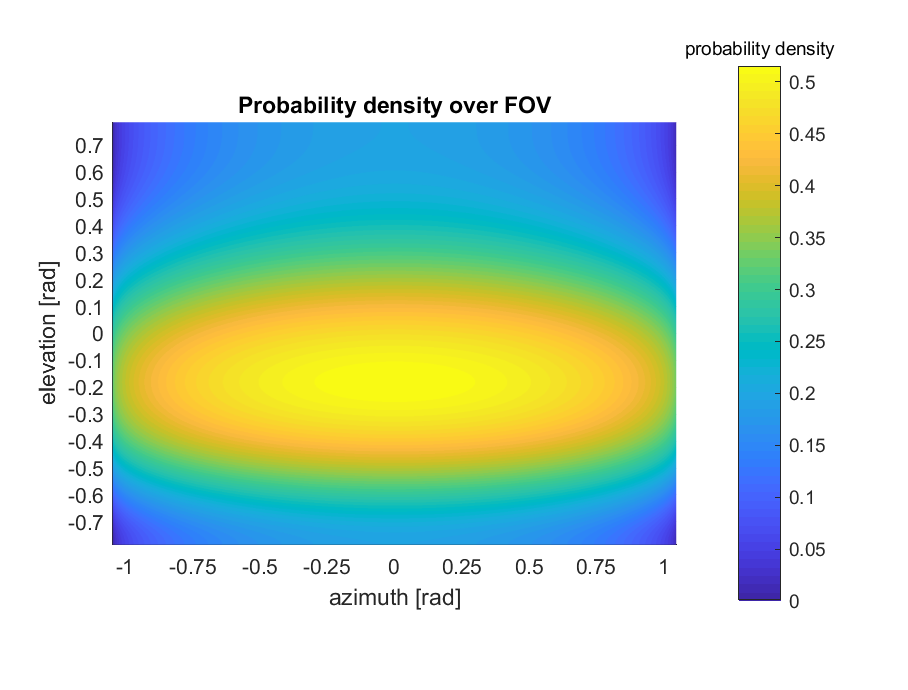
\includegraphics[width=0.9\linewidth]{fig/betapdf.eps}
\caption[Example of stochastic actor output]{Probability density of picking ray, with specific azimuth and elevation.}
\label{fig:stochaction}
\end{figure}

\subsection{Comparison of methods}
Several methods were tried. Unfortunately, most of the methods do not perform well in the Lidar-gym environment. The DQL had the worst performance. That is probably caused by the extremly large action space. The workaround made in formula \eqref{eq:dql}, did not help the agent to converge. Continuous DDPG agent also did not converge successfully. For DDPG agent is hard to change direction of rays efficiently in subsequent timestamps and it often makes several same actions in a row, that degrades performance a lot. Only the stochastic agent was able to outperform a random agent. Summary of agents performances is made in Figure \ref{fig:roc}. It turns out that it is very difficult to get satisfying results. Stochastic agent converges, but it does not use any kind of advanced strategy. Output of the DDPG actor does not even allow him to make any sophisticated action. Therefore were also conducted experiments with an extended stochastic agent, which used beta distribution for each ray separately, but with no significant success. Another advantage of simple stochastic agent is its scalability. This agent can be adjusted to the large environment much easier than any other used agent. Parameters used for these agents are described in Table \ref{tab:params}.

\clearpage

\begin{table}[h!]
  \centering
  \begin{tabular}{*{2}{c}}
    \toprule
    Parameter & Value \\
    \midrule
    $\gamma$ & 0.09 \\
    $\lambda_{c}$ & 0.001 \\
    $\lambda_{a}$ & 0.0001 \\
    $\tau$ & 0.01 \\
    Memory size & 4096 \\
    Batch size & 8 \\
    \bottomrule
  \end{tabular}
  \caption[Learning parameters]{Parameters used for learning. DQN uses $\lambda = \lambda_{c}$}
  \label{tab:params}
\end{table}

\begin{figure}[h!]
\centering
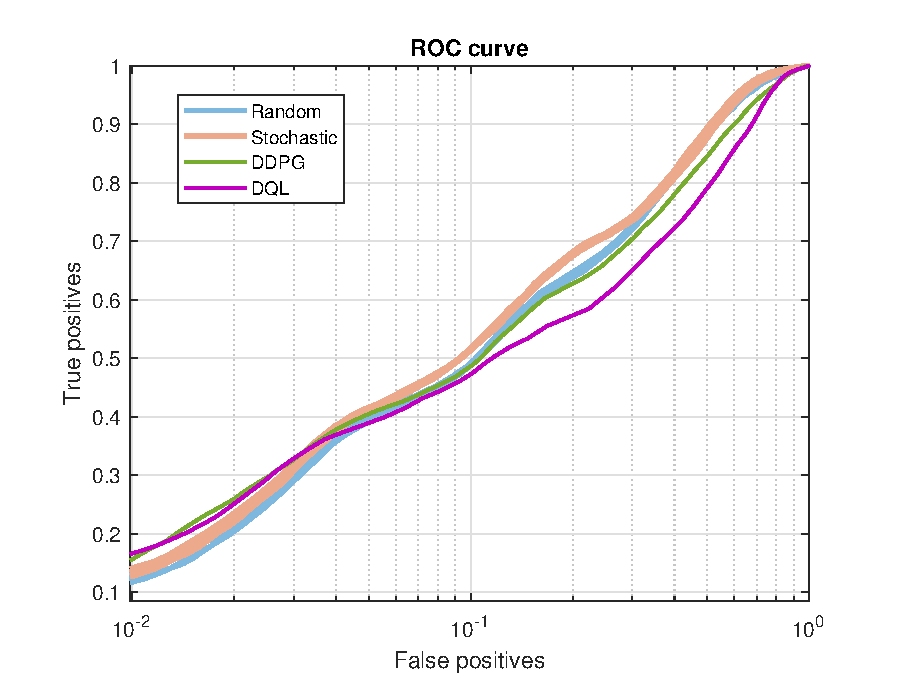
\includegraphics[width=1\linewidth]{fig/roc.eps}
\caption[ROC curves comparison]{False positives were calculated using ground truth map and true positives using all voxels, which could be possibly hit by sensor. Five different evaluations are displayed for non-deterministic agents.}
\label{fig:roc}
\end{figure}

\clearpage



\clearpage

\fancyhead[LO,LE]{CONCLUSION}
\section{Conclusion}

BLAH BLAH BLAH
\cleardoublepage

\fancyhead[LO,LE]{LIST OF REFERENCES}
% the list of all literature should be supplied in main.bib
\bibliographystyle{unsrt}
\bibliography{main}{}
\clearpage

\appendices
\fancyhead[LO,LE]{APPENDIX}
\section{CD Content}

In Table~\ref{tab:obsah} are listed names of all root directories on CD.

\vspace{1cm}
\begin{table}[!htb]
\centering
\begin{tabular}{lp{10cm}}
\textbf{Directory name} & \textbf{Description} \\

\hline
thesis & the thesis in pdf format \\
ctu\_thesis & latex source codes \\
lidar-gym & OpenAI gym environment \\
\hline
\end{tabular}
\caption{CD Content}
\label{tab:obsah}
\end{table}

\cleardoublepage

\section{List of abbreviations}\label{ape:abbreviations}

In Table \ref{table:abbreviations} are listed abbreviations used in this thesis.

\begin{table}[!htb]
\centering
\begin{tabular}{ll}
\textbf{Abbreviation} & \textbf{Meaning} \\
\hline
\textbf{CNN} & Convolutional neural network \\
\hline
\textbf{DDPG} & Deep deterministic policy gradients \\
\hline
\textbf{DQN} & Deep Q-learning \\
\hline
\textbf{MDP} & Markov decision process \\
\hline
\textbf{RL} & Reinforcement learning \\
\hline
\textbf{ReLu} & Rectified linear unit \\
\hline
\textbf{TD} & Temporal difference \\
\hline
\end{tabular}
\caption{Lists of abbreviations}
\label{table:abbreviations}
\end{table}
\cleardoublepage

\end{document}
